
\documentclass[12pt]{article}
\usepackage[margin=1in]{geometry}
\usepackage[portuguese]{babel}
% Core packages
\usepackage{amsmath,amssymb}
\usepackage{tikz-cd}
\usepackage{multicol}
\usepackage{ragged2e}

% Paragraphs
\setlength{\parindent}{0pt}
\setlength{\parskip}{1\baselineskip}

\title{Empréstimos e Planos de Amortização}
\author{Instituto Federal do Amazonas \\ Disciplina: Matemática Financeira \\ Profa. Me. Dulcineide Pereira dos Santos\\ Prova elaborada por: Joao Victor, Joseph Cesar e Everton de Souza \\ Atividade (total: \textbf{10,00} pontos)}
\date{10 de junho de 2026}


\begin{document}
\large
\maketitle
\noindent Aluno(a): \rule{10cm}{0.4pt} \hfill Nota: \rule{2cm}{0.4pt}


\begin{enumerate}
    \justifying
    \item \textbf{[1,5]} Maximiliano e Tânia são amigos que amam os animais. Eles decidiram oferecer serviços de refeições prontas de alimentação natural crua e cozida para pets. Para iniciar o negócio, os sócios tomaram emprestados R\$ 8.000,00 a juros de 5\% ao mês, divididos em dezesseis meses ao regime de amortização constante. Determine o valor da oitava prestação. 
    %\textcolor{red}{R\$ 725,00}

    \noindent R: \rule{6cm}{0.4pt}
    \item \textbf{[2,5]} Um cliente comprou um imóvel no valor de R\$ 600.000,00. Para isso, pagou 20\% desse valor de entrada, em dezembro de 2023, e financiou o restante em prestações mensais no Sistema de Amortização Constante (SAC), a uma taxa de 0,5\% ao mês, em um prazo de 20 anos, com a primeira prestação para janeiro de 2024 e a última para dezembro de 2043. A prestação mensal é composta de juros, amortização e uma taxa fixa de R\$ 100,00 mensais (no ano de 2024) referente ao seguro. Considere que todas as prestações desse financiamento sejam pagas dentro do prazo. Determine a soma das 12 primeiras prestações (referentes ao período de janeiro de 2024 a dezembro de 2024) a serem pagas por esse cliente. \noindent R: \rule{6cm}{0.4pt} %R$ 53.340,00.
    %\textcolor{red}{R\$ 53.340,00}%.

    \item 
    \textbf{[2,0]} Um banco financia R\$ 5.000,00 a um cliente, com base na tabela Price e a juros de 15\% a.a., para serem devolvidos em 10 meses. Construa o plano de amortização dessa dívida.

    \item 
    \textbf{[1,5]} Um empréstimo de \$ 30\,000,00 deve ser pago em 4 parcelas trimestrais iguais, com juros de 10\% em cada trimestre. Construa o plano de amortização.

    \item 
    \textbf{[1,0]} Uma revendedora de motos divulga a seguinte propaganda de venda:
    $$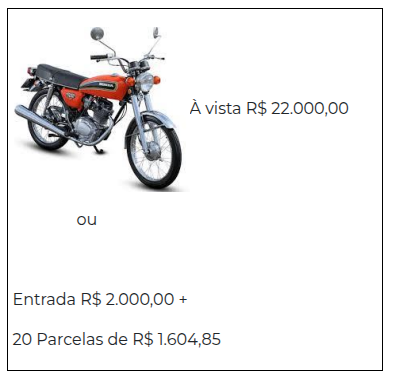
\includegraphics[scale=0.6]{imagem_1.png}$$    

    $$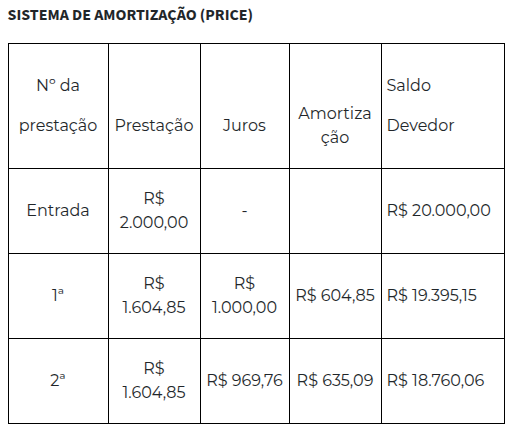
\includegraphics[scale=0.5]{imagem_2.png}$$ \\ A revendedora apresenta aos compradores uma tabela que utiliza o sistema francês de financiamento (Tabela Price), conforme resumo dos 3 primeiros pagamentos apresentados acima, ao lado da propaganda. Considerando os dados fornecidos na tabela, determine o valor do saldo devedor, em reais, após o pagamento da 3ª prestação. \\ 
    %\textcolor{red}{R\$ 18.093,21}
    \noindent R: \rule{6cm}{0.4pt} %

    \item 
    \textbf{[1,5]} Acerca dos custos dos empréstimos e seus sistemas de amortização, julgue o item que se segue. Considere-se que tenha sido financiado pelo sistema americano de amortização um bem no valor de R\$ 335.000, a ser pago em três anos, com taxa de juros de 10\% ao ano, e que, nesse financiamento, os juros tenham sido pagos periodicamente a cada ano. Com base nessa situação hipotética, é correto afirmar que a tabela subsequente fornece a planilha financeira correta desse financiamento.

    $$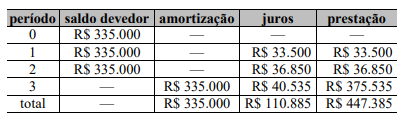
\includegraphics[scale=0.8]{questao_1.png}$$

    \noindent ( ) Certo \quad (  ) Errado %\textcolor{red}{( x ) Errado}   %errado
    
\end{enumerate}


\end{document}

